\documentclass[1p]{elsarticle_modified}
%\bibliographystyle{elsarticle-num}

%\usepackage[colorlinks]{hyperref}
%\usepackage{abbrmath_seonhwa} %\Abb, \Ascr, \Acal ,\Abf, \Afrak
\usepackage{amsfonts}
\usepackage{amssymb}
\usepackage{amsmath}
\usepackage{amsthm}
\usepackage{scalefnt}
\usepackage{amsbsy}
\usepackage{kotex}
\usepackage{caption}
\usepackage{subfig}
\usepackage{color}
\usepackage{graphicx}
\usepackage{xcolor} %% white, black, red, green, blue, cyan, magenta, yellow
\usepackage{float}
\usepackage{setspace}
\usepackage{hyperref}

\usepackage{tikz}
\usetikzlibrary{arrows}

\usepackage{multirow}
\usepackage{array} % fixed length table
\usepackage{hhline}

%%%%%%%%%%%%%%%%%%%%%
\makeatletter
\renewcommand*\env@matrix[1][\arraystretch]{%
	\edef\arraystretch{#1}%
	\hskip -\arraycolsep
	\let\@ifnextchar\new@ifnextchar
	\array{*\c@MaxMatrixCols c}}
\makeatother %https://tex.stackexchange.com/questions/14071/how-can-i-increase-the-line-spacing-in-a-matrix
%%%%%%%%%%%%%%%

\usepackage[normalem]{ulem}

\newcommand{\msout}[1]{\ifmmode\text{\sout{\ensuremath{#1}}}\else\sout{#1}\fi}
%SOURCE: \msout is \stkout macro in https://tex.stackexchange.com/questions/20609/strikeout-in-math-mode

\newcommand{\cancel}[1]{
	\ifmmode
	{\color{red}\msout{#1}}
	\else
	{\color{red}\sout{#1}}
	\fi
}

\newcommand{\add}[1]{
	{\color{blue}\uwave{#1}}
}

\newcommand{\replace}[2]{
	\ifmmode
	{\color{red}\msout{#1}}{\color{blue}\uwave{#2}}
	\else
	{\color{red}\sout{#1}}{\color{blue}\uwave{#2}}
	\fi
}

\newcommand{\Sol}{\mathcal{S}} %segment
\newcommand{\D}{D} %diagram
\newcommand{\A}{\mathcal{A}} %arc


%%%%%%%%%%%%%%%%%%%%%%%%%%%%%5 test

\def\sl{\operatorname{\textup{SL}}(2,\Cbb)}
\def\psl{\operatorname{\textup{PSL}}(2,\Cbb)}
\def\quan{\mkern 1mu \triangleright \mkern 1mu}

\theoremstyle{definition}
\newtheorem{thm}{Theorem}[section]
\newtheorem{prop}[thm]{Proposition}
\newtheorem{lem}[thm]{Lemma}
\newtheorem{ques}[thm]{Question}
\newtheorem{cor}[thm]{Corollary}
\newtheorem{defn}[thm]{Definition}
\newtheorem{exam}[thm]{Example}
\newtheorem{rmk}[thm]{Remark}
\newtheorem{alg}[thm]{Algorithm}

\newcommand{\I}{\sqrt{-1}}
\begin{document}

%\begin{frontmatter}
%
%\title{Boundary parabolic representations of knots up to 8 crossings}
%
%%% Group authors per affiliation:
%\author{Yunhi Cho} 
%\address{Department of Mathematics, University of Seoul, Seoul, Korea}
%\ead{yhcho@uos.ac.kr}
%
%
%\author{Seonhwa Kim} %\fnref{s_kim}}
%\address{Center for Geometry and Physics, Institute for Basic Science, Pohang, 37673, Korea}
%\ead{ryeona17@ibs.re.kr}
%
%\author{Hyuk Kim}
%\address{Department of Mathematical Sciences, Seoul National University, Seoul 08826, Korea}
%\ead{hyukkim@snu.ac.kr}
%
%\author{Seokbeom Yoon}
%\address{Department of Mathematical Sciences, Seoul National University, Seoul, 08826,  Korea}
%\ead{sbyoon15@snu.ac.kr}
%
%\begin{abstract}
%We find all boundary parabolic representation of knots up to 8 crossings.
%
%\end{abstract}
%\begin{keyword}
%    \MSC[2010] 57M25 
%\end{keyword}
%
%\end{frontmatter}

%\linenumbers
%\tableofcontents
%
\newcommand\colored[1]{\textcolor{white}{\rule[-0.35ex]{0.8em}{1.4ex}}\kern-0.8em\color{red} #1}%
%\newcommand\colored[1]{\textcolor{white}{ #1}\kern-2.17ex	\textcolor{white}{ #1}\kern-1.81ex	\textcolor{white}{ #1}\kern-2.15ex\color{red}#1	}

{\Large $\underline{12n_{0011}~(K12n_{0011})}$}

\setlength{\tabcolsep}{10pt}
\renewcommand{\arraystretch}{1.6}
\vspace{1cm}\begin{tabular}{m{100pt}>{\centering\arraybackslash}m{274pt}}
\multirow{5}{120pt}{
	\centering
	\includegraphics[width=112pt]{../../../GIT/diagram.site/Diagrams/png/2100_12n_0011.png}\\
\ \ \ A knot diagram\footnotemark}&
\allowdisplaybreaks
\textbf{Linearized knot diagam} \\
\cline{2-2}
 &
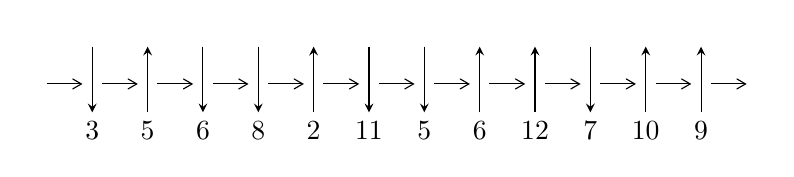
\begin{tikzpicture}[x=20pt, y=17pt]
	% nodes
	\node (C0) at (0, 0) {};
	\node (C1) at (1, 0) {};
	\node (C1U) at (1, +1) {};
	\node (C1D) at (1, -1) {3};

	\node (C2) at (2, 0) {};
	\node (C2U) at (2, +1) {};
	\node (C2D) at (2, -1) {5};

	\node (C3) at (3, 0) {};
	\node (C3U) at (3, +1) {};
	\node (C3D) at (3, -1) {6};

	\node (C4) at (4, 0) {};
	\node (C4U) at (4, +1) {};
	\node (C4D) at (4, -1) {8};

	\node (C5) at (5, 0) {};
	\node (C5U) at (5, +1) {};
	\node (C5D) at (5, -1) {2};

	\node (C6) at (6, 0) {};
	\node (C6U) at (6, +1) {};
	\node (C6D) at (6, -1) {11};

	\node (C7) at (7, 0) {};
	\node (C7U) at (7, +1) {};
	\node (C7D) at (7, -1) {5};

	\node (C8) at (8, 0) {};
	\node (C8U) at (8, +1) {};
	\node (C8D) at (8, -1) {6};

	\node (C9) at (9, 0) {};
	\node (C9U) at (9, +1) {};
	\node (C9D) at (9, -1) {12};

	\node (C10) at (10, 0) {};
	\node (C10U) at (10, +1) {};
	\node (C10D) at (10, -1) {7};

	\node (C11) at (11, 0) {};
	\node (C11U) at (11, +1) {};
	\node (C11D) at (11, -1) {10};

	\node (C12) at (12, 0) {};
	\node (C12U) at (12, +1) {};
	\node (C12D) at (12, -1) {9};
	\node (C13) at (13, 0) {};

	% arrows
	\draw[->,>={angle 60}]
	(C0) edge (C1) (C1) edge (C2) (C2) edge (C3) (C3) edge (C4) (C4) edge (C5) (C5) edge (C6) (C6) edge (C7) (C7) edge (C8) (C8) edge (C9) (C9) edge (C10) (C10) edge (C11) (C11) edge (C12) (C12) edge (C13) ;	\draw[->,>=stealth]
	(C1U) edge (C1D) (C2D) edge (C2U) (C3U) edge (C3D) (C4U) edge (C4D) (C5D) edge (C5U) (C6U) edge (C6D) (C7U) edge (C7D) (C8D) edge (C8U) (C9D) edge (C9U) (C10U) edge (C10D) (C11D) edge (C11U) (C12D) edge (C12U) ;
	\end{tikzpicture} \\
\hhline{~~} \\& 
\textbf{Solving Sequence} \\ \cline{2-2} 
 &
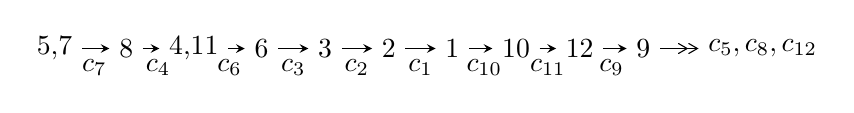
\begin{tikzpicture}[x=23pt, y=7pt]
	% node
	\node (A0) at (-1/8, 0) {5,7};
	\node (A1) at (1, 0) {8};
	\node (A2) at (33/16, 0) {4,11};
	\node (A3) at (25/8, 0) {6};
	\node (A4) at (33/8, 0) {3};
	\node (A5) at (41/8, 0) {2};
	\node (A6) at (49/8, 0) {1};
	\node (A7) at (57/8, 0) {10};
	\node (A8) at (65/8, 0) {12};
	\node (A9) at (73/8, 0) {9};
	\node (C1) at (1/2, -1) {$c_{7}$};
	\node (C2) at (3/2, -1) {$c_{4}$};
	\node (C3) at (21/8, -1) {$c_{6}$};
	\node (C4) at (29/8, -1) {$c_{3}$};
	\node (C5) at (37/8, -1) {$c_{2}$};
	\node (C6) at (45/8, -1) {$c_{1}$};
	\node (C7) at (53/8, -1) {$c_{10}$};
	\node (C8) at (61/8, -1) {$c_{11}$};
	\node (C9) at (69/8, -1) {$c_{9}$};
	\node (A10) at (11, 0) {$c_{5},c_{8},c_{12}$};

	% edge
	\draw[->,>=stealth]	
	(A0) edge (A1) (A1) edge (A2) (A2) edge (A3) (A3) edge (A4) (A4) edge (A5) (A5) edge (A6) (A6) edge (A7) (A7) edge (A8) (A8) edge (A9) ;
	\draw[->>,>={angle 60}]	
	(A9) edge (A10);
\end{tikzpicture} \\ 

\end{tabular} \\

\footnotetext{
The image of knot diagram is generated by the software ``\textbf{Draw programme}" developed by Andrew Bartholomew(\url{http://www.layer8.co.uk/maths/draw/index.htm\#Running-draw}), where we modified some parts for our purpose(\url{https://github.com/CATsTAILs/LinksPainter}).
}\phantom \\ \newline 
\centering \textbf{Ideals for irreducible components\footnotemark of $X_{\text{par}}$} 
 
\begin{align*}
I^u_{1}&=\langle 
-5.71616\times10^{69} u^{37}+1.11175\times10^{70} u^{36}+\cdots+3.33891\times10^{72} b+1.88016\times10^{72},\\
\phantom{I^u_{1}}&\phantom{= \langle  }4.07046\times10^{70} u^{37}-5.21445\times10^{70} u^{36}+\cdots+1.33556\times10^{73} a-1.19377\times10^{73},\\
\phantom{I^u_{1}}&\phantom{= \langle  }u^{38}- u^{37}+\cdots+128 u+256\rangle \\
\\
I^v_{1}&=\langle 
a,\;18 v^7-26 v^6+12 v^5-78 v^4+71 v^3+30 v^2+19 b+6 v-2,\;v^8-2 v^7+v^6-4 v^5+6 v^4+v^3-2 v^2- v+1\rangle \\
\end{align*}
\raggedright * 2 irreducible components of $\dim_{\mathbb{C}}=0$, with total 46 representations.\\
\footnotetext{All coefficients of polynomials are rational numbers. But the coefficients are sometimes approximated in decimal forms when there is not enough margin.}
\newpage
\renewcommand{\arraystretch}{1}
\centering \section*{I. $I^u_{1}= \langle -5.72\times10^{69} u^{37}+1.11\times10^{70} u^{36}+\cdots+3.34\times10^{72} b+1.88\times10^{72},\;4.07\times10^{70} u^{37}-5.21\times10^{70} u^{36}+\cdots+1.34\times10^{73} a-1.19\times10^{73},\;u^{38}- u^{37}+\cdots+128 u+256 \rangle$}
\flushleft \textbf{(i) Arc colorings}\\
\begin{tabular}{m{7pt} m{180pt} m{7pt} m{180pt} }
\flushright $a_{5}=$&$\begin{pmatrix}0\\u\end{pmatrix}$ \\
\flushright $a_{7}=$&$\begin{pmatrix}1\\0\end{pmatrix}$ \\
\flushright $a_{8}=$&$\begin{pmatrix}1\\u^2\end{pmatrix}$ \\
\flushright $a_{4}=$&$\begin{pmatrix}u\\u^3+u\end{pmatrix}$ \\
\flushright $a_{11}=$&$\begin{pmatrix}-0.00304774 u^{37}+0.00390431 u^{36}+\cdots-2.13353 u+0.893835\\0.00171198 u^{37}-0.00332968 u^{36}+\cdots-0.453692 u-0.563107\end{pmatrix}$ \\
\flushright $a_{6}=$&$\begin{pmatrix}0.00130957 u^{37}+0.00189335 u^{36}+\cdots-1.90974 u+2.64338\\-0.00109847 u^{37}+0.00183184 u^{36}+\cdots-0.794202 u-0.211610\end{pmatrix}$ \\
\flushright $a_{3}=$&$\begin{pmatrix}0.00359002 u^{37}-0.00745031 u^{36}+\cdots+4.56333 u-0.957202\\0.00112443 u^{37}-0.000480799 u^{36}+\cdots+0.826261 u+0.801763\end{pmatrix}$ \\
\flushright $a_{2}=$&$\begin{pmatrix}0.00359002 u^{37}-0.00745031 u^{36}+\cdots+4.56333 u-0.957202\\0.00209211 u^{37}-0.000172711 u^{36}+\cdots+0.401334 u+1.79000\end{pmatrix}$ \\
\flushright $a_{1}=$&$\begin{pmatrix}-0.000952567 u^{37}-0.000976781 u^{36}+\cdots+1.86076 u-2.03505\\0.000357004 u^{37}+0.000916565 u^{36}+\cdots-0.0489786 u+0.608337\end{pmatrix}$ \\
\flushright $a_{10}=$&$\begin{pmatrix}-0.00133576 u^{37}+0.000574632 u^{36}+\cdots-2.58722 u+0.330728\\0.00171198 u^{37}-0.00332968 u^{36}+\cdots-0.453692 u-0.563107\end{pmatrix}$ \\
\flushright $a_{12}=$&$\begin{pmatrix}0.000400109 u^{37}+0.00305192 u^{36}+\cdots-3.11755 u+1.84992\\0.00136835 u^{37}-0.000426605 u^{36}+\cdots-0.970171 u-0.257429\end{pmatrix}$ \\
\flushright $a_{9}=$&$\begin{pmatrix}-0.00313189 u^{37}+0.00425632 u^{36}+\cdots-0.691749 u+0.425379\\-0.00175985 u^{37}+0.00256836 u^{36}+\cdots+0.691063 u-0.518052\end{pmatrix}$\\&\end{tabular}
\flushleft \textbf{(ii) Obstruction class $= -1$}\\~\\
\flushleft \textbf{(iii) Cusp Shapes $= -0.0107565 u^{37}+0.0115767 u^{36}+\cdots-16.3471 u-2.84993$}\\~\\
\newpage\renewcommand{\arraystretch}{1}
\flushleft \textbf{(iv) u-Polynomials at the component}\newline \\
\begin{tabular}{m{50pt}|m{274pt}}
Crossings & \hspace{64pt}u-Polynomials at each crossing \\
\hline $$\begin{aligned}c_{1}\end{aligned}$$&$\begin{aligned}
&u^{38}+9 u^{37}+\cdots+15 u+1
\end{aligned}$\\
\hline $$\begin{aligned}c_{2},c_{5}\end{aligned}$$&$\begin{aligned}
&u^{38}+5 u^{37}+\cdots+3 u+1
\end{aligned}$\\
\hline $$\begin{aligned}c_{3}\end{aligned}$$&$\begin{aligned}
&u^{38}-5 u^{37}+\cdots+90147 u+15489
\end{aligned}$\\
\hline $$\begin{aligned}c_{4},c_{7}\end{aligned}$$&$\begin{aligned}
&u^{38}- u^{37}+\cdots+128 u+256
\end{aligned}$\\
\hline $$\begin{aligned}c_{6},c_{10}\end{aligned}$$&$\begin{aligned}
&u^{38}+3 u^{37}+\cdots- u+1
\end{aligned}$\\
\hline $$\begin{aligned}c_{8}\end{aligned}$$&$\begin{aligned}
&u^{38}+3 u^{37}+\cdots+u+1
\end{aligned}$\\
\hline $$\begin{aligned}c_{9},c_{11},c_{12}\end{aligned}$$&$\begin{aligned}
&u^{38}-11 u^{37}+\cdots-11 u+1
\end{aligned}$\\
\hline
\end{tabular}\\~\\
\newpage\renewcommand{\arraystretch}{1}
\flushleft \textbf{(v) Riley Polynomials at the component}\newline \\
\begin{tabular}{m{50pt}|m{274pt}}
Crossings & \hspace{64pt}Riley Polynomials at each crossing \\
\hline $$\begin{aligned}c_{1}\end{aligned}$$&$\begin{aligned}
&y^{38}+45 y^{37}+\cdots+91 y+1
\end{aligned}$\\
\hline $$\begin{aligned}c_{2},c_{5}\end{aligned}$$&$\begin{aligned}
&y^{38}+9 y^{37}+\cdots+15 y+1
\end{aligned}$\\
\hline $$\begin{aligned}c_{3}\end{aligned}$$&$\begin{aligned}
&y^{38}+81 y^{37}+\cdots+7556564583 y+239909121
\end{aligned}$\\
\hline $$\begin{aligned}c_{4},c_{7}\end{aligned}$$&$\begin{aligned}
&y^{38}+45 y^{37}+\cdots+344064 y+65536
\end{aligned}$\\
\hline $$\begin{aligned}c_{6},c_{10}\end{aligned}$$&$\begin{aligned}
&y^{38}+11 y^{37}+\cdots+11 y+1
\end{aligned}$\\
\hline $$\begin{aligned}c_{8}\end{aligned}$$&$\begin{aligned}
&y^{38}-65 y^{37}+\cdots+11 y+1
\end{aligned}$\\
\hline $$\begin{aligned}c_{9},c_{11},c_{12}\end{aligned}$$&$\begin{aligned}
&y^{38}+35 y^{37}+\cdots+131 y+1
\end{aligned}$\\
\hline
\end{tabular}\\~\\
\newpage\flushleft \textbf{(vi) Complex Volumes and Cusp Shapes}
$$\begin{array}{c|c|c}  
\text{Solutions to }I^u_{1}& \I (\text{vol} + \sqrt{-1}CS) & \text{Cusp shape}\\
 \hline 
\begin{aligned}
u &= \phantom{-}0.801035 + 0.695463 I \\
a &= \phantom{-}0.79350 - 1.46806 I \\
b &= \phantom{-}0.025706 + 0.900927 I\end{aligned}
 & \phantom{-}2.72429 - 1.49580 I & \phantom{-}6.88383 + 3.00756 I \\ \hline\begin{aligned}
u &= \phantom{-}0.801035 - 0.695463 I \\
a &= \phantom{-}0.79350 + 1.46806 I \\
b &= \phantom{-}0.025706 - 0.900927 I\end{aligned}
 & \phantom{-}2.72429 + 1.49580 I & \phantom{-}6.88383 - 3.00756 I \\ \hline\begin{aligned}
u &= -0.213839 + 1.135170 I \\
a &= -0.421285 - 0.668176 I \\
b &= \phantom{-}0.784497 + 0.822982 I\end{aligned}
 & -4.44084 + 0.93436 I & -3.64457 - 1.20353 I \\ \hline\begin{aligned}
u &= -0.213839 - 1.135170 I \\
a &= -0.421285 + 0.668176 I \\
b &= \phantom{-}0.784497 - 0.822982 I\end{aligned}
 & -4.44084 - 0.93436 I & -3.64457 + 1.20353 I \\ \hline\begin{aligned}
u &= -1.159340 + 0.148885 I \\
a &= -1.361450 + 0.030633 I \\
b &= -0.708036 + 0.833117 I\end{aligned}
 & -1.60611 - 0.16717 I & -2.00112 - 0.51691 I \\ \hline\begin{aligned}
u &= -1.159340 - 0.148885 I \\
a &= -1.361450 - 0.030633 I \\
b &= -0.708036 - 0.833117 I\end{aligned}
 & -1.60611 + 0.16717 I & -2.00112 + 0.51691 I \\ \hline\begin{aligned}
u &= -0.358418 + 0.734904 I \\
a &= \phantom{-}1.30197 + 2.31889 I \\
b &= -0.136751 - 0.822464 I\end{aligned}
 & \phantom{-}1.16926 - 3.17447 I & \phantom{-}5.84543 + 3.28927 I \\ \hline\begin{aligned}
u &= -0.358418 - 0.734904 I \\
a &= \phantom{-}1.30197 - 2.31889 I \\
b &= -0.136751 + 0.822464 I\end{aligned}
 & \phantom{-}1.16926 + 3.17447 I & \phantom{-}5.84543 - 3.28927 I \\ \hline\begin{aligned}
u &= \phantom{-}0.183194 + 1.207340 I \\
a &= \phantom{-}0.229775 + 1.020680 I \\
b &= \phantom{-}0.677081 - 0.878596 I\end{aligned}
 & -0.69910 + 2.61127 I & \phantom{-}1.65431 - 3.00859 I \\ \hline\begin{aligned}
u &= \phantom{-}0.183194 - 1.207340 I \\
a &= \phantom{-}0.229775 - 1.020680 I \\
b &= \phantom{-}0.677081 + 0.878596 I\end{aligned}
 & -0.69910 - 2.61127 I & \phantom{-}1.65431 + 3.00859 I\\
 \hline 
 \end{array}$$\newpage$$\begin{array}{c|c|c}  
\text{Solutions to }I^u_{1}& \I (\text{vol} + \sqrt{-1}CS) & \text{Cusp shape}\\
 \hline 
\begin{aligned}
u &= \phantom{-}0.083408 + 1.218640 I \\
a &= \phantom{-}0.31884 - 1.60799 I \\
b &= \phantom{-}0.755833 + 0.932426 I\end{aligned}
 & -4.10208 - 6.74360 I & -2.53206 + 6.49784 I \\ \hline\begin{aligned}
u &= \phantom{-}0.083408 - 1.218640 I \\
a &= \phantom{-}0.31884 + 1.60799 I \\
b &= \phantom{-}0.755833 - 0.932426 I\end{aligned}
 & -4.10208 + 6.74360 I & -2.53206 - 6.49784 I \\ \hline\begin{aligned}
u &= \phantom{-}1.262280 + 0.110410 I \\
a &= -1.310290 + 0.231935 I \\
b &= -0.705134 - 0.909841 I\end{aligned}
 & -1.36537 - 5.58839 I & -0.94341 + 6.04268 I \\ \hline\begin{aligned}
u &= \phantom{-}1.262280 - 0.110410 I \\
a &= -1.310290 - 0.231935 I \\
b &= -0.705134 + 0.909841 I\end{aligned}
 & -1.36537 + 5.58839 I & -0.94341 - 6.04268 I \\ \hline\begin{aligned}
u &= -0.533596 + 0.416988 I \\
a &= -0.970594 - 0.091212 I \\
b &= -0.856400 + 0.889730 I\end{aligned}
 & -7.10344 + 1.95919 I & -5.95273 - 5.24866 I \\ \hline\begin{aligned}
u &= -0.533596 - 0.416988 I \\
a &= -0.970594 + 0.091212 I \\
b &= -0.856400 - 0.889730 I\end{aligned}
 & -7.10344 - 1.95919 I & -5.95273 + 5.24866 I \\ \hline\begin{aligned}
u &= \phantom{-}0.525705 + 0.422944 I \\
a &= -0.981407 - 0.165229 I \\
b &= -0.842922 + 0.929719 I\end{aligned}
 & -6.97962 + 4.35433 I & -5.02974 + 0.36700 I \\ \hline\begin{aligned}
u &= \phantom{-}0.525705 - 0.422944 I \\
a &= -0.981407 + 0.165229 I \\
b &= -0.842922 - 0.929719 I\end{aligned}
 & -6.97962 - 4.35433 I & -5.02974 - 0.36700 I \\ \hline\begin{aligned}
u &= -0.437849 + 0.512305 I \\
a &= \phantom{-}0.779426 + 0.427405 I \\
b &= \phantom{-}0.391315 - 0.479189 I\end{aligned}
 & -0.621022 + 1.245300 I & -4.66633 - 4.67696 I \\ \hline\begin{aligned}
u &= -0.437849 - 0.512305 I \\
a &= \phantom{-}0.779426 - 0.427405 I \\
b &= \phantom{-}0.391315 + 0.479189 I\end{aligned}
 & -0.621022 - 1.245300 I & -4.66633 + 4.67696 I\\
 \hline 
 \end{array}$$\newpage$$\begin{array}{c|c|c}  
\text{Solutions to }I^u_{1}& \I (\text{vol} + \sqrt{-1}CS) & \text{Cusp shape}\\
 \hline 
\begin{aligned}
u &= \phantom{-}0.517700 + 0.295561 I \\
a &= \phantom{-}0.655146 + 0.862409 I \\
b &= \phantom{-}0.360279 - 0.813117 I\end{aligned}
 & \phantom{-}0.31192 + 1.82341 I & \phantom{-}0.28789 - 3.69490 I \\ \hline\begin{aligned}
u &= \phantom{-}0.517700 - 0.295561 I \\
a &= \phantom{-}0.655146 - 0.862409 I \\
b &= \phantom{-}0.360279 + 0.813117 I\end{aligned}
 & \phantom{-}0.31192 - 1.82341 I & \phantom{-}0.28789 + 3.69490 I \\ \hline\begin{aligned}
u &= -0.304409 + 0.498073 I \\
a &= \phantom{-}1.074620 - 0.335260 I \\
b &= -0.237341 - 0.266456 I\end{aligned}
 & -0.29515 + 1.55177 I & -2.39420 - 5.36172 I \\ \hline\begin{aligned}
u &= -0.304409 - 0.498073 I \\
a &= \phantom{-}1.074620 + 0.335260 I \\
b &= -0.237341 + 0.266456 I\end{aligned}
 & -0.29515 - 1.55177 I & -2.39420 + 5.36172 I \\ \hline\begin{aligned}
u &= -0.54647 + 1.64480 I \\
a &= \phantom{-}0.0641318 + 0.0863728 I \\
b &= \phantom{-}0.904591 + 0.748202 I\end{aligned}
 & \phantom{-}3.59603 + 6.55252 I & \phantom{-0.000000 } 0 \\ \hline\begin{aligned}
u &= -0.54647 - 1.64480 I \\
a &= \phantom{-}0.0641318 - 0.0863728 I \\
b &= \phantom{-}0.904591 - 0.748202 I\end{aligned}
 & \phantom{-}3.59603 - 6.55252 I & \phantom{-0.000000 } 0 \\ \hline\begin{aligned}
u &= \phantom{-}0.34197 + 1.69965 I \\
a &= \phantom{-}0.1067440 + 0.0256339 I \\
b &= \phantom{-}0.889409 - 0.715074 I\end{aligned}
 & \phantom{-}4.26554 + 0.00326 I & \phantom{-0.000000 } 0 \\ \hline\begin{aligned}
u &= \phantom{-}0.34197 - 1.69965 I \\
a &= \phantom{-}0.1067440 - 0.0256339 I \\
b &= \phantom{-}0.889409 + 0.715074 I\end{aligned}
 & \phantom{-}4.26554 - 0.00326 I & \phantom{-0.000000 } 0 \\ \hline\begin{aligned}
u &= -0.13035 + 1.76573 I \\
a &= -0.0597378 - 0.0404559 I \\
b &= -0.799015 - 0.032415 I\end{aligned}
 & \phantom{-}8.11017 + 3.32648 I & \phantom{-0.000000 } 0 \\ \hline\begin{aligned}
u &= -0.13035 - 1.76573 I \\
a &= -0.0597378 + 0.0404559 I \\
b &= -0.799015 + 0.032415 I\end{aligned}
 & \phantom{-}8.11017 - 3.32648 I & \phantom{-0.000000 } 0\\
 \hline 
 \end{array}$$\newpage$$\begin{array}{c|c|c}  
\text{Solutions to }I^u_{1}& \I (\text{vol} + \sqrt{-1}CS) & \text{Cusp shape}\\
 \hline 
\begin{aligned}
u &= \phantom{-}0.62652 + 1.70416 I \\
a &= \phantom{-}1.02467 - 1.15119 I \\
b &= \phantom{-}0.788823 + 1.027640 I\end{aligned}
 & \phantom{-}4.47409 - 12.81500 I & \phantom{-0.000000 } 0 \\ \hline\begin{aligned}
u &= \phantom{-}0.62652 - 1.70416 I \\
a &= \phantom{-}1.02467 + 1.15119 I \\
b &= \phantom{-}0.788823 - 1.027640 I\end{aligned}
 & \phantom{-}4.47409 + 12.81500 I & \phantom{-0.000000 } 0 \\ \hline\begin{aligned}
u &= -0.43365 + 1.79825 I \\
a &= \phantom{-}0.88940 + 1.14293 I \\
b &= \phantom{-}0.765371 - 1.032090 I\end{aligned}
 & \phantom{-}5.25384 + 6.12703 I & \phantom{-0.000000 } 0 \\ \hline\begin{aligned}
u &= -0.43365 - 1.79825 I \\
a &= \phantom{-}0.88940 - 1.14293 I \\
b &= \phantom{-}0.765371 + 1.032090 I\end{aligned}
 & \phantom{-}5.25384 - 6.12703 I & \phantom{-0.000000 } 0 \\ \hline\begin{aligned}
u &= \phantom{-}0.32788 + 1.90698 I \\
a &= -0.52275 + 1.62668 I \\
b &= -0.300160 - 1.097060 I\end{aligned}
 & \phantom{-}11.67940 - 7.06576 I & \phantom{-0.000000 } 0 \\ \hline\begin{aligned}
u &= \phantom{-}0.32788 - 1.90698 I \\
a &= -0.52275 - 1.62668 I \\
b &= -0.300160 + 1.097060 I\end{aligned}
 & \phantom{-}11.67940 + 7.06576 I & \phantom{-0.000000 } 0 \\ \hline\begin{aligned}
u &= -0.05179 + 1.95040 I \\
a &= -0.36069 - 1.63993 I \\
b &= -0.257145 + 1.102200 I\end{aligned}
 & \phantom{-}11.94710 + 0.17151 I & \phantom{-0.000000 } 0 \\ \hline\begin{aligned}
u &= -0.05179 - 1.95040 I \\
a &= -0.36069 + 1.63993 I \\
b &= -0.257145 - 1.102200 I\end{aligned}
 & \phantom{-}11.94710 - 0.17151 I & \phantom{-0.000000 } 0\\
 \hline 
 \end{array}$$\newpage\newpage\renewcommand{\arraystretch}{1}
\centering \section*{II. $I^v_{1}= \langle a,\;18 v^7-26 v^6+\cdots+19 b-2,\;v^8-2 v^7+v^6-4 v^5+6 v^4+v^3-2 v^2- v+1 \rangle$}
\flushleft \textbf{(i) Arc colorings}\\
\begin{tabular}{m{7pt} m{180pt} m{7pt} m{180pt} }
\flushright $a_{5}=$&$\begin{pmatrix}v\\0\end{pmatrix}$ \\
\flushright $a_{7}=$&$\begin{pmatrix}1\\0\end{pmatrix}$ \\
\flushright $a_{8}=$&$\begin{pmatrix}1\\0\end{pmatrix}$ \\
\flushright $a_{4}=$&$\begin{pmatrix}v\\0\end{pmatrix}$ \\
\flushright $a_{11}=$&$\begin{pmatrix}0\\-0.947368 v^{7}+1.36842 v^{6}+\cdots-0.315789 v+0.105263\end{pmatrix}$ \\
\flushright $a_{6}=$&$\begin{pmatrix}1\\-1.26316 v^{7}+2.15789 v^{6}+\cdots-0.421053 v+1.47368\end{pmatrix}$ \\
\flushright $a_{3}=$&$\begin{pmatrix}0.368421 v^{7}-0.421053 v^{6}+\cdots+0.789474 v-1.26316\\0.263158 v^{7}-0.157895 v^{6}+\cdots+2.42105 v-0.473684\end{pmatrix}$ \\
\flushright $a_{2}=$&$\begin{pmatrix}0.0526316 v^{7}+0.368421 v^{6}+\cdots+0.684211 v-0.894737\\0.263158 v^{7}-0.157895 v^{6}+\cdots+2.42105 v-0.473684\end{pmatrix}$ \\
\flushright $a_{1}=$&$\begin{pmatrix}-1\\1.26316 v^{7}-2.15789 v^{6}+\cdots+0.421053 v-1.47368\end{pmatrix}$ \\
\flushright $a_{10}=$&$\begin{pmatrix}-0.947368 v^{7}+1.36842 v^{6}+\cdots-0.315789 v+0.105263\\-0.947368 v^{7}+1.36842 v^{6}+\cdots-0.315789 v+0.105263\end{pmatrix}$ \\
\flushright $a_{12}=$&$\begin{pmatrix}-0.789474 v^{7}+1.47368 v^{6}+\cdots-0.263158 v+2.42105\\-1.73684 v^{7}+2.84211 v^{6}+\cdots-0.578947 v+2.52632\end{pmatrix}$ \\
\flushright $a_{9}=$&$\begin{pmatrix}1.26316 v^{7}-2.15789 v^{6}+\cdots+0.421053 v-0.473684\\0.473684 v^{7}-0.684211 v^{6}+\cdots+0.157895 v+1.94737\end{pmatrix}$\\&\end{tabular}
\flushleft \textbf{(ii) Obstruction class $= 1$}\\~\\
\flushleft \textbf{(iii) Cusp Shapes $= -\frac{23}{19} v^7-\frac{9}{19} v^6+\frac{67}{19} v^5+\frac{49}{19} v^4+\frac{94}{19} v^3-\frac{298}{19} v^2+\frac{43}{19} v+\frac{11}{19}$}\\~\\
\newpage\renewcommand{\arraystretch}{1}
\flushleft \textbf{(iv) u-Polynomials at the component}\newline \\
\begin{tabular}{m{50pt}|m{274pt}}
Crossings & \hspace{64pt}u-Polynomials at each crossing \\
\hline $$\begin{aligned}c_{1},c_{3},c_{5}\end{aligned}$$&$\begin{aligned}
&(u^2- u+1)^4
\end{aligned}$\\
\hline $$\begin{aligned}c_{2}\end{aligned}$$&$\begin{aligned}
&(u^2+u+1)^4
\end{aligned}$\\
\hline $$\begin{aligned}c_{4},c_{7}\end{aligned}$$&$\begin{aligned}
&u^8
\end{aligned}$\\
\hline $$\begin{aligned}c_{6}\end{aligned}$$&$\begin{aligned}
&(u^4+u^3+u^2+1)^2
\end{aligned}$\\
\hline $$\begin{aligned}c_{8},c_{11},c_{12}\end{aligned}$$&$\begin{aligned}
&(u^4- u^3+3 u^2-2 u+1)^2
\end{aligned}$\\
\hline $$\begin{aligned}c_{9}\end{aligned}$$&$\begin{aligned}
&(u^4+u^3+3 u^2+2 u+1)^2
\end{aligned}$\\
\hline $$\begin{aligned}c_{10}\end{aligned}$$&$\begin{aligned}
&(u^4- u^3+u^2+1)^2
\end{aligned}$\\
\hline
\end{tabular}\\~\\
\newpage\renewcommand{\arraystretch}{1}
\flushleft \textbf{(v) Riley Polynomials at the component}\newline \\
\begin{tabular}{m{50pt}|m{274pt}}
Crossings & \hspace{64pt}Riley Polynomials at each crossing \\
\hline $$\begin{aligned}c_{1},c_{2},c_{3}\\c_{5}\end{aligned}$$&$\begin{aligned}
&(y^2+y+1)^4
\end{aligned}$\\
\hline $$\begin{aligned}c_{4},c_{7}\end{aligned}$$&$\begin{aligned}
&y^8
\end{aligned}$\\
\hline $$\begin{aligned}c_{6},c_{10}\end{aligned}$$&$\begin{aligned}
&(y^4+y^3+3 y^2+2 y+1)^2
\end{aligned}$\\
\hline $$\begin{aligned}c_{8},c_{9},c_{11}\\c_{12}\end{aligned}$$&$\begin{aligned}
&(y^4+5 y^3+7 y^2+2 y+1)^2
\end{aligned}$\\
\hline
\end{tabular}\\~\\
\newpage\flushleft \textbf{(vi) Complex Volumes and Cusp Shapes}
$$\begin{array}{c|c|c}  
\text{Solutions to }I^v_{1}& \I (\text{vol} + \sqrt{-1}CS) & \text{Cusp shape}\\
 \hline 
\begin{aligned}
v &= \phantom{-}0.576953 + 0.283088 I \\
a &= \phantom{-0.000000 } 0 \\
b &= -0.851808 - 0.911292 I\end{aligned}
 & -6.79074 - 1.13408 I & -2.09237 - 2.48762 I \\ \hline\begin{aligned}
v &= \phantom{-}0.576953 - 0.283088 I \\
a &= \phantom{-0.000000 } 0 \\
b &= -0.851808 + 0.911292 I\end{aligned}
 & -6.79074 + 1.13408 I & -2.09237 + 2.48762 I \\ \hline\begin{aligned}
v &= -0.533637 + 0.358112 I \\
a &= \phantom{-0.000000 } 0 \\
b &= -0.851808 - 0.911292 I\end{aligned}
 & -6.79074 - 5.19385 I & -2.75261 + 7.88731 I \\ \hline\begin{aligned}
v &= -0.533637 - 0.358112 I \\
a &= \phantom{-0.000000 } 0 \\
b &= -0.851808 + 0.911292 I\end{aligned}
 & -6.79074 + 5.19385 I & -2.75261 - 7.88731 I \\ \hline\begin{aligned}
v &= \phantom{-}1.54112 + 0.21492 I \\
a &= \phantom{-0.000000 } 0 \\
b &= \phantom{-}0.351808 - 0.720342 I\end{aligned}
 & \phantom{-}0.211005 - 0.614778 I & \phantom{-}2.55284 - 0.89520 I \\ \hline\begin{aligned}
v &= \phantom{-}1.54112 - 0.21492 I \\
a &= \phantom{-0.000000 } 0 \\
b &= \phantom{-}0.351808 + 0.720342 I\end{aligned}
 & \phantom{-}0.211005 + 0.614778 I & \phantom{-}2.55284 + 0.89520 I \\ \hline\begin{aligned}
v &= -0.58443 + 1.44211 I \\
a &= \phantom{-0.000000 } 0 \\
b &= \phantom{-}0.351808 + 0.720342 I\end{aligned}
 & \phantom{-}0.21101 - 3.44499 I & -2.20786 + 6.97475 I \\ \hline\begin{aligned}
v &= -0.58443 - 1.44211 I \\
a &= \phantom{-0.000000 } 0 \\
b &= \phantom{-}0.351808 - 0.720342 I\end{aligned}
 & \phantom{-}0.21101 + 3.44499 I & -2.20786 - 6.97475 I\\
 \hline 
 \end{array}$$\newpage
\newpage\renewcommand{\arraystretch}{1}
\centering \section*{ III. u-Polynomials}
\begin{tabular}{m{50pt}|m{274pt}}
Crossings & \hspace{64pt}u-Polynomials at each crossing \\
\hline $$\begin{aligned}c_{1}\end{aligned}$$&$\begin{aligned}
&((u^2- u+1)^4)(u^{38}+9 u^{37}+\cdots+15 u+1)
\end{aligned}$\\
\hline $$\begin{aligned}c_{2}\end{aligned}$$&$\begin{aligned}
&((u^2+u+1)^4)(u^{38}+5 u^{37}+\cdots+3 u+1)
\end{aligned}$\\
\hline $$\begin{aligned}c_{3}\end{aligned}$$&$\begin{aligned}
&((u^2- u+1)^4)(u^{38}-5 u^{37}+\cdots+90147 u+15489)
\end{aligned}$\\
\hline $$\begin{aligned}c_{4},c_{7}\end{aligned}$$&$\begin{aligned}
&u^8(u^{38}- u^{37}+\cdots+128 u+256)
\end{aligned}$\\
\hline $$\begin{aligned}c_{5}\end{aligned}$$&$\begin{aligned}
&((u^2- u+1)^4)(u^{38}+5 u^{37}+\cdots+3 u+1)
\end{aligned}$\\
\hline $$\begin{aligned}c_{6}\end{aligned}$$&$\begin{aligned}
&((u^4+u^3+u^2+1)^2)(u^{38}+3 u^{37}+\cdots- u+1)
\end{aligned}$\\
\hline $$\begin{aligned}c_{8}\end{aligned}$$&$\begin{aligned}
&((u^4- u^3+3 u^2-2 u+1)^2)(u^{38}+3 u^{37}+\cdots+u+1)
\end{aligned}$\\
\hline $$\begin{aligned}c_{9}\end{aligned}$$&$\begin{aligned}
&((u^4+u^3+3 u^2+2 u+1)^2)(u^{38}-11 u^{37}+\cdots-11 u+1)
\end{aligned}$\\
\hline $$\begin{aligned}c_{10}\end{aligned}$$&$\begin{aligned}
&((u^4- u^3+u^2+1)^2)(u^{38}+3 u^{37}+\cdots- u+1)
\end{aligned}$\\
\hline $$\begin{aligned}c_{11},c_{12}\end{aligned}$$&$\begin{aligned}
&((u^4- u^3+3 u^2-2 u+1)^2)(u^{38}-11 u^{37}+\cdots-11 u+1)
\end{aligned}$\\
\hline
\end{tabular}\newpage\renewcommand{\arraystretch}{1}
\centering \section*{ IV. Riley Polynomials}
\begin{tabular}{m{50pt}|m{274pt}}
Crossings & \hspace{64pt}Riley Polynomials at each crossing \\
\hline $$\begin{aligned}c_{1}\end{aligned}$$&$\begin{aligned}
&((y^2+y+1)^4)(y^{38}+45 y^{37}+\cdots+91 y+1)
\end{aligned}$\\
\hline $$\begin{aligned}c_{2},c_{5}\end{aligned}$$&$\begin{aligned}
&((y^2+y+1)^4)(y^{38}+9 y^{37}+\cdots+15 y+1)
\end{aligned}$\\
\hline $$\begin{aligned}c_{3}\end{aligned}$$&$\begin{aligned}
&((y^2+y+1)^4)(y^{38}+81 y^{37}+\cdots+7.55656\times10^{9} y+2.39909\times10^{8})
\end{aligned}$\\
\hline $$\begin{aligned}c_{4},c_{7}\end{aligned}$$&$\begin{aligned}
&y^8(y^{38}+45 y^{37}+\cdots+344064 y+65536)
\end{aligned}$\\
\hline $$\begin{aligned}c_{6},c_{10}\end{aligned}$$&$\begin{aligned}
&((y^4+y^3+3 y^2+2 y+1)^2)(y^{38}+11 y^{37}+\cdots+11 y+1)
\end{aligned}$\\
\hline $$\begin{aligned}c_{8}\end{aligned}$$&$\begin{aligned}
&((y^4+5 y^3+7 y^2+2 y+1)^2)(y^{38}-65 y^{37}+\cdots+11 y+1)
\end{aligned}$\\
\hline $$\begin{aligned}c_{9},c_{11},c_{12}\end{aligned}$$&$\begin{aligned}
&((y^4+5 y^3+7 y^2+2 y+1)^2)(y^{38}+35 y^{37}+\cdots+131 y+1)
\end{aligned}$\\
\hline
\end{tabular}
\vskip 2pc
\end{document}